\section*{Math 202A - HW11 - Dan Davison - \texttt{ddavison@berkeley.edu}}

\begin{mdframed}
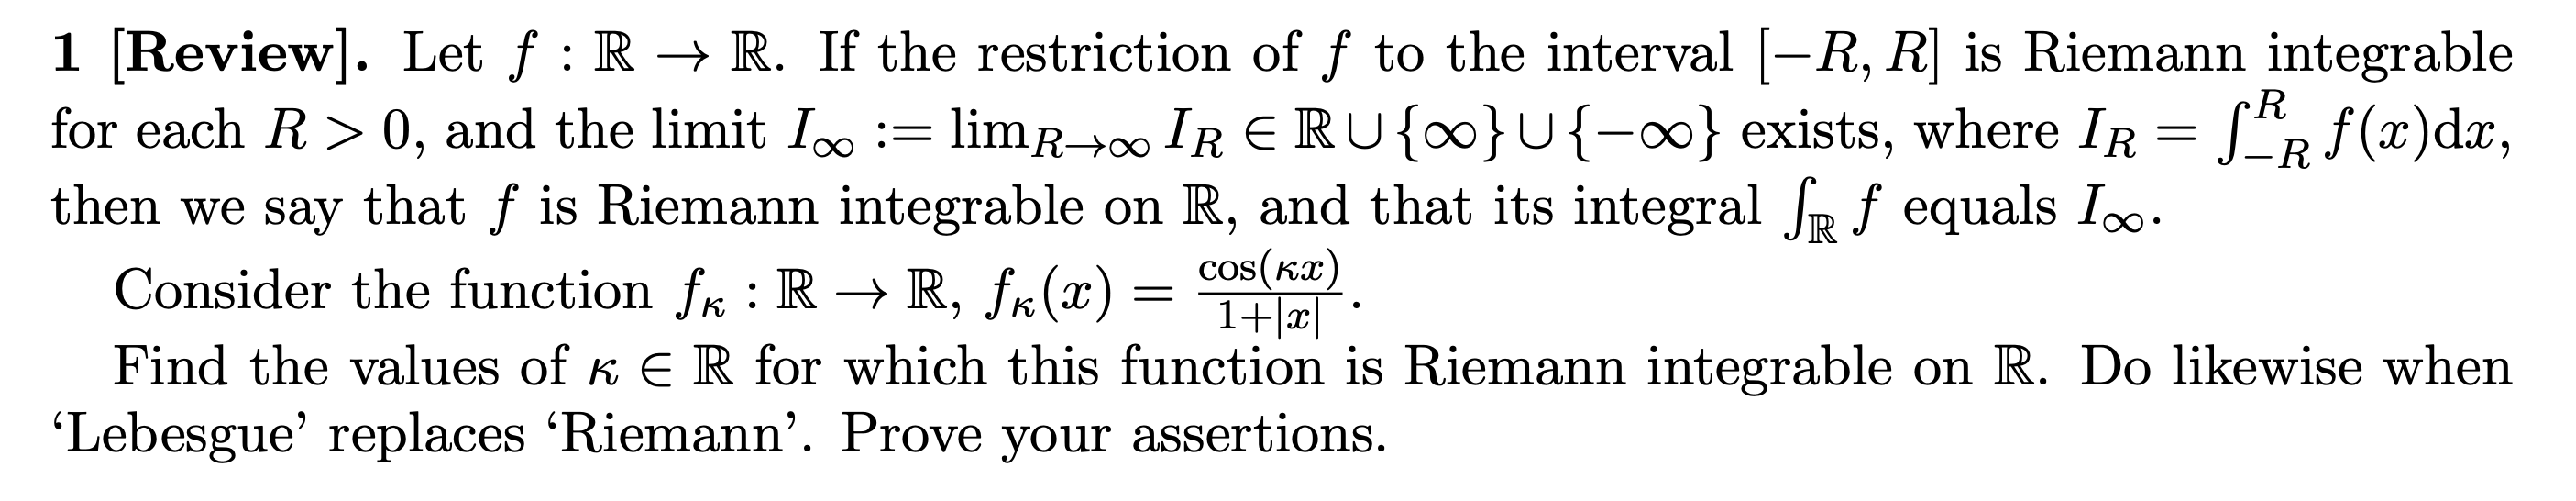
\includegraphics[width=400pt]{img/analysis--berkeley-202a-hw11-8650.png}
\end{mdframed}

\begin{lemma}[Dirichlet's test for improper integrals]
  Let $I = \int_a^\infty f(x) g(x) \dx$ where $\int$ denotes the Riemann integral. Then $I$ converges if all
  the following are true
  \begin{enumerate}
  \item $f$ is continuous on $[a, \infty]$
  \item $\int_a^x f(t) \dt$ is bounded on $[a, \infty]$
  \item $g$ is differentiable on $[a, \infty]$ with $g' \leq 0$ and $\lim_{x\to\infty} g(x) = 0$.
  \end{enumerate}
\end{lemma}

\begin{proof}
  Note that $f_\kappa$ is an even function, therefore (hint from @ankit in
  Slack) $\int_{-R}^R f_{\kappa}(x) \dx = 2\int_{0}^R f_\kappa(x)$ and
  therefore $I_\infty = \frac{1}{2}\int_0^\infty f_{\kappa}(x) \dx$, if this limit (in the upper bound of the
  integral) exists.

  We now (hint from Piazza) invoke Dirichlet's test with $a = 0$, $g(x) = 1/(1 + x)$,
  and $f(x) = \cos(\kappa x)$, where these variable names refer to the statement in the lemma. We see that $f$
  is continuous on $[0, \infty]$ as required; we see that $\int_0^x f_{\kappa}(t) \dt = \sin(\kappa t)$ is
  bounded on $[0, \infty]$; and we see that $g$ is differentiable on $[0, \infty]$ with $g'(x) = -1/(1 + x)^2$
  and that $g(x) \to 0$ as $x \to \infty$. Therefore we conclude that $\int_0^\infty f_{\kappa}(x) \dx$
  converges and therefore that $f_{\kappa}$ is Riemann integrable for all $\kappa$.

  By definition, $f_{\kappa}$ is Lebesgue integrable if $\int_{-\infty}^\infty |f_{\kappa}| < \infty$.
  Since $|f_{\kappa}|$ is even and non-negative, $f_{\kappa}$ is Lebesgue integrable if and only
  if $\int_{0}^\infty |f_{\kappa}| < \infty$.

  Note that (by considering the graphs of $|\cos(\kappa x)|$ and $1/(1 + x)$)
  \begin{align*}
    \int_{0}^\infty |f_{\kappa}|
    = \int_0^\infty \frac{|\cos(\kappa x)|}{1 + x}
    > \(\int_0^{2\pi}|\cos(\kappa x)|\) \sum_{n=1}^\infty \frac{1}{1 + 2n\pi}.
  \end{align*}
  Clearly $\int_0^{2\pi}|\cos(\kappa x)| > 0$. But $\sum_{n=1}^\infty \frac{1}{1 + 2n\pi}$ is a divergent
  series, therefore $f_{\kappa}$ is not Lebesgue integrable for any value of $\kappa$.
\end{proof}


\begin{mdframed}
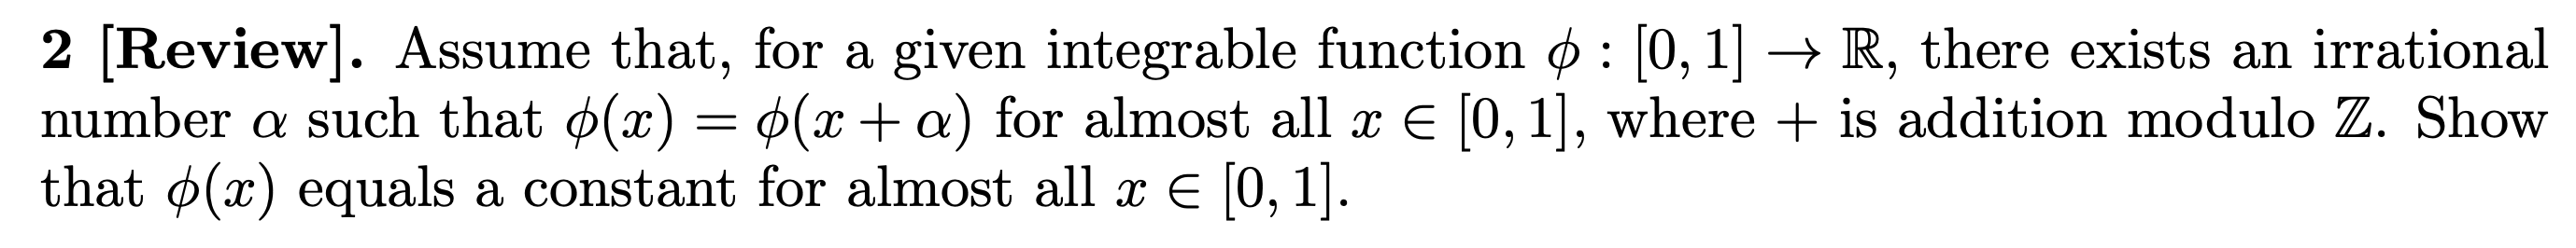
\includegraphics[width=400pt]{img/analysis--berkeley-202a-hw11-b6a3.png}
\end{mdframed}

This is true because the orbit of the map $x \mapsto x + a$ is dense in $[0, 1]$. We basically just need to show that.

We must show that $\phi(x)$ equals a constant for almost all $x$.

Why should that be? Why, for example, can't each orbit have its own constant value?


\begin{proof}
  Let $\tau: [0, 1) \to [0, 1)$ be the map defined by $x \mapsto x + \alpha \mod \Z$, and for $x \in [0, 1)$
  define the sequence $(r_n(x)) = x, \tau(x), \tau^2(x), \ldots$, and
  let $\orb(x) := \big\{r_n(x) ~:~ n \in \N\big\}$ be the orbit of $x$ under $\tau$. Recall from HW2 and HW6
  that for each $x \in [0, 1)$ the sequence $(r_n(x))$ is non-repeating, the corresponding orbit $\orb(x)$ is
  dense in $[0, 1]$, and each orbit is disjoint from every other orbit. Thus each orbit is a countable set and
  there are uncountably many distinct orbits.

  We have that the set of points $x$ at which $\phi(\tau(x)) = \phi(x)$ has measure $1$. Therefore we have the
  following qualitative picture: there are uncountably many disjoint orbits and each orbit is associated with a
  sequence $\phi(x), \phi(\tau(x)), \phi(\tau^2(x)), \ldots$. The set of points at which this sequence changes
  value has measure $0$.

  We must use the fact that $\phi$ is integrable to show that $\phi$ is constant a.e.

  Let $\eps > 0$ and let $g: [0, 1] \to \R$ be a continuous function such that
  \begin{align*}
    \int |g - \phi| < \eps.
  \end{align*}






  Let $\eps > 0$. According to Lusin's theorem there exists a closed set $F \subseteq [0, 1]$
  with $m(F) > 1- \eps$ such that $\phi|_F$ is continuous. So let $F \subseteq [0, 1]$ be such that $m(F) = 1$
  and $\phi|_F$ is continuous.

  Note that $F$ is uncountable and therefore it contains points from uncountably many orbits.


  Probabilistic view:

  - Pick $x$. It is a member of some orbit and has some value $\phi(x)$. We have $Pr(\phi(x + \alpha) = \phi(x)) = 1$.

  - Suppose the claim is not true. Then there exist $c$ and $d$ such that $m(\phi = c) = p_c > 0$ and $m(\phi = d) = p_d > 0$.

  - Pick $x$. With probability $p_c$ we have $\phi(x) = c$ and also $\phi(x + \alpha) = c$.










  Why might $\phi$ be constant a.e.?

  - Each orbit is countable, so if one orbit is constant, that's just a measure zero set.

  - Similarly, if every orbit is constant, but they all have different values that's not constant a.e.

  - What we need to show is something more like that all orbits ``start​'' with the same value

\end{proof}


\begin{mdframed}
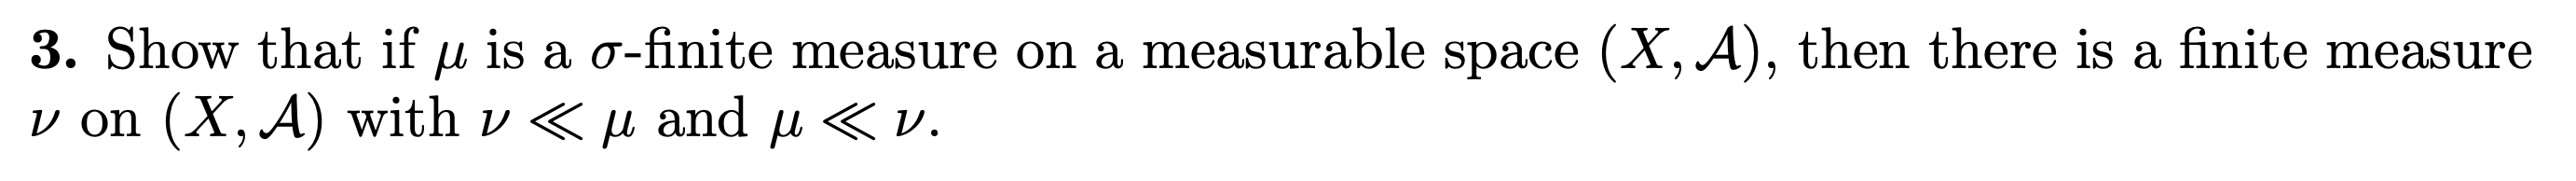
\includegraphics[width=400pt]{img/analysis--berkeley-202a-hw11-3704.png}
\end{mdframed}


\begin{mdframed}
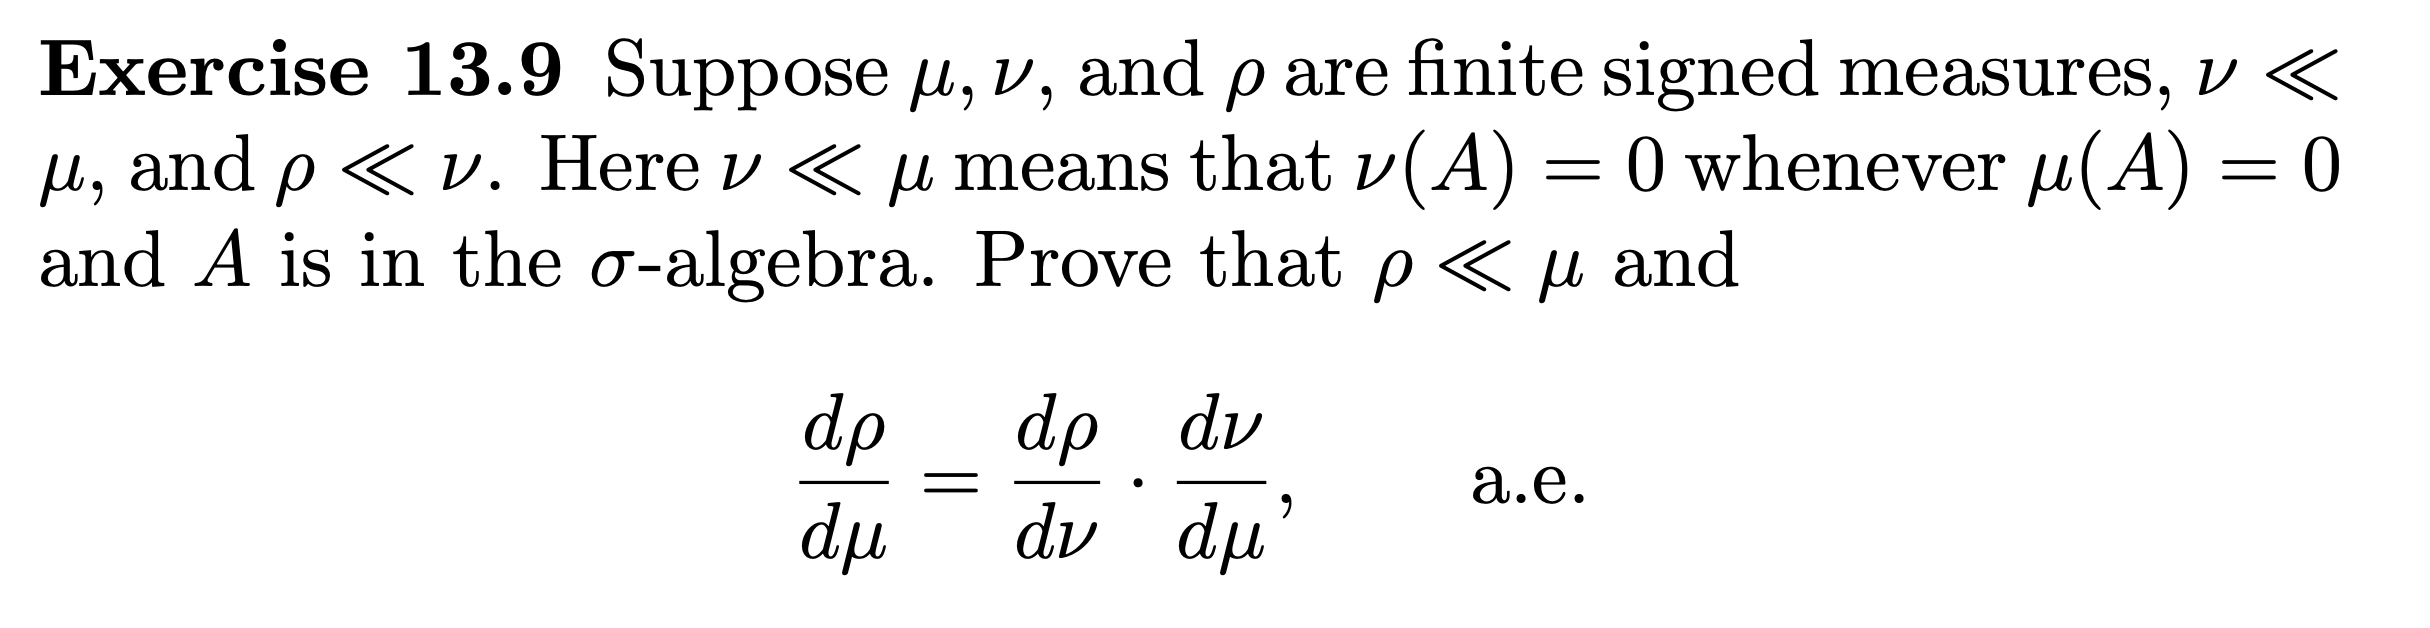
\includegraphics[width=400pt]{img/analysis--berkeley-202a-hw11-f2c0.png}
\end{mdframed}


\begin{claim*}
  $\rho \ll \mu$
\end{claim*}
\begin{proof}
  We must show that $\rho(A) = 0$ whenever $\mu(A) = 0$ and $A$ is in the $\sigma$-algebra.

  Let $A$ be in the $\sigma$-algebra such that $\mu(A) = 0$. Then $\nu(A) = 0$, since $\nu \ll \mu$.
  Therefore $\rho(A) = 0$, since $\rho \ll \nu$.
\end{proof}

\begin{claim*}
  \begin{align*}
    \frac{\d\nu}{\d\lambda} = \frac{\d\nu}{\d\mu}\frac{\d\mu}{\d\lambda} \ae
  \end{align*}
\end{claim*}

\begin{proof}
  By definition, $\frac{\d\nu}{\d\lambda}$ is a function such that for any measurable set $E$
  \begin{align*}
    \nu(E) = \int_E \frac{\d\nu}{\d\lambda} \d\lambda.
  \end{align*}
  We will first show that the function $\frac{\d\nu}{\d\mu}\frac{\d\mu}{\d\lambda}$ also serves as a derivative
  of $\nu$ with respect to $\lambda$, i.e. that for any measurable set $E$
  \begin{align*}
    \nu(E) = \int_E \frac{\d\nu}{\d\mu}\frac{\d\mu}{\d\lambda} \d\lambda.
  \end{align*}
  Let $E$ be a measurable set.

  First note that

  Write $f = \frac{\d\nu}{\d\mu}$ and let $f_n$ be a sequence of increasing simple functions converging
  pointwise to $f$. Let $F$ be a measurable set and note that
  \begin{align*}
    \int_E \ind_F \d\mu
    = \mu(E \cap F)
    = \int_{E \cap F} \frac{\d\mu}{\d\lambda} \d\lambda
    = \int_E \ind_F \frac{\d\mu}{\d\lambda} \d\lambda.
  \end{align*}
  Therefore by linearity of the integral
  \begin{align*}
    \int_E f_n \d\mu = \int_{E} f_n \frac{\d\mu}{\d\lambda}\d\lambda,
  \end{align*}
  and taking the limit as $n \to \infty$ (\red{I think I should be using MCT somewhere, could you tell me where?})
  \begin{align*}
    \int_E f \d\mu = \int_{E} f \frac{\d\mu}{\d\lambda}\d\lambda.
  \end{align*}
  Substituting its definition $\frac{\d\nu}{\d\mu}$ in place of the symbol $f$ we have
  \begin{align*}
    \int_E \frac{\d\nu}{\d\mu} \d\mu
    = \nu(E)
    = \int_E \frac{\d\nu}{\d\lambda} \d\lambda
    = \int_{E} \frac{\d\nu}{\d\mu} \frac{\d\mu}{\d\lambda}\d\lambda.
  \end{align*}

  Therefore
  \begin{align*}
    \int_E \frac{\d\nu}{\d\lambda}  - \frac{\d\nu}{\d\mu}\frac{\d\mu}{\d\lambda} \d\lambda = 0,
  \end{align*}
  and therefore
  \begin{align*}
    \frac{\d\nu}{\d\lambda} = \frac{\d\nu}{\d\mu}\frac{\d\mu}{\d\lambda} \ae
  \end{align*}
\end{proof}

\begin{mdframed}
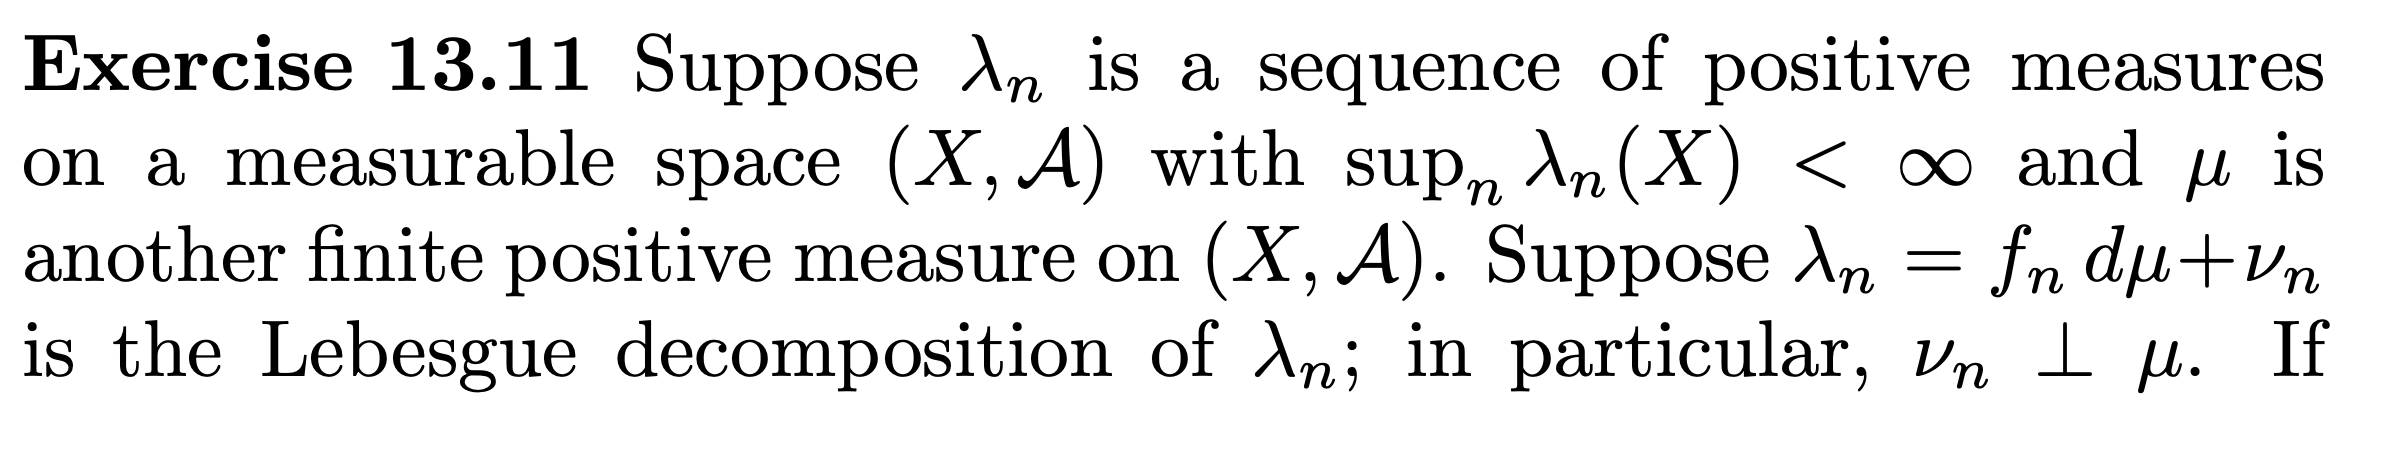
\includegraphics[width=400pt]{img/analysis--berkeley-202a-hw11-c5a4.png}
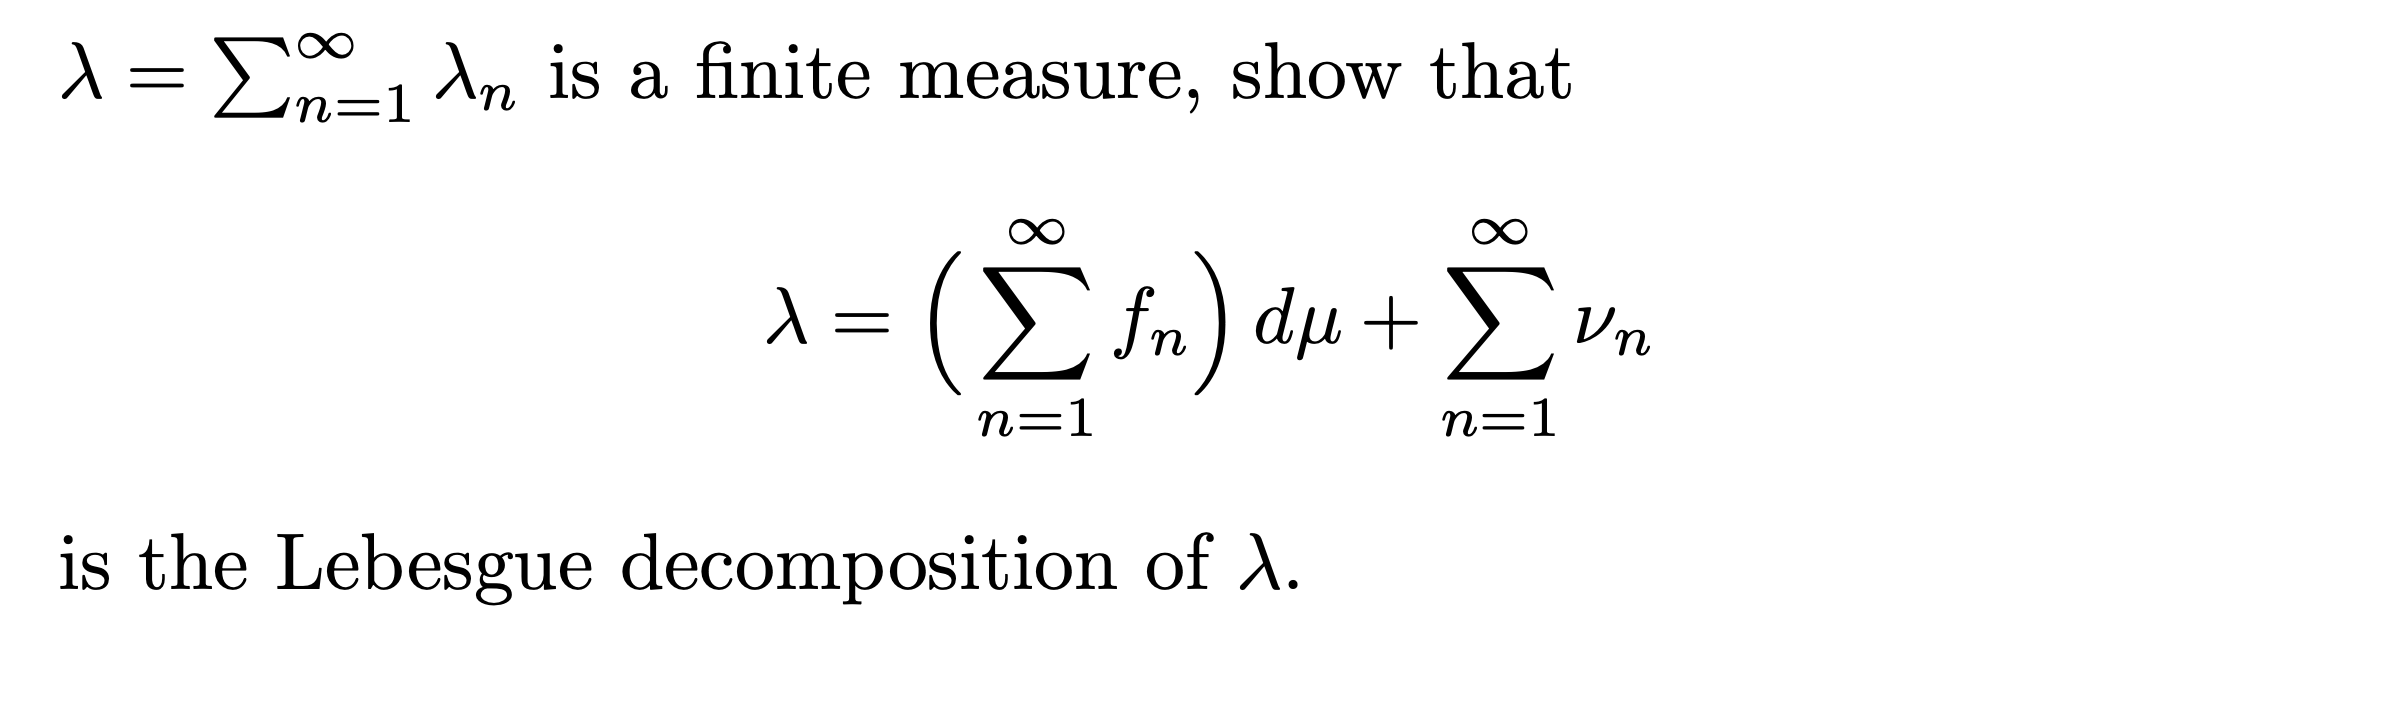
\includegraphics[width=400pt]{img/analysis--berkeley-202a-hw11-3974.png}
\end{mdframed}